\documentclass{tufte-handout}

\title{CMPT 419/726 --- Machine Learning}

\author[Salehen Shovon Rahman]{Salehen Shovon Rahman}

%\date{28 March 2010} % without \date command, current date is supplied

%\geometry{showframe} % display margins for debugging page layout

\usepackage{graphicx} % allow embedded images
  \setkeys{Gin}{width=\linewidth,totalheight=\textheight,keepaspectratio}
  \graphicspath{{graphics/}} % set of paths to search for images
\usepackage{amsmath}  % extended mathematics
\usepackage{booktabs} % book-quality tables
\usepackage{units}    % non-stacked fractions and better unit spacing
\usepackage{multicol} % multiple column layout facilities
\usepackage{lipsum}   % filler text
\usepackage{fancyvrb} % extended verbatim environments
\usepackage{tcolorbox}
  \fvset{fontsize=\normalsize}% default font size for fancy-verbatim environments

% Standardize command font styles and environments
\newcommand{\doccmd}[1]{\texttt{\textbackslash#1}}% command name -- adds backslash automatically
\newcommand{\docopt}[1]{\ensuremath{\langle}\textrm{\textit{#1}}\ensuremath{\rangle}}% optional command argument
\newcommand{\docarg}[1]{\textrm{\textit{#1}}}% (required) command argument
\newcommand{\docenv}[1]{\textsf{#1}}% environment name
\newcommand{\docpkg}[1]{\texttt{#1}}% package name
\newcommand{\doccls}[1]{\texttt{#1}}% document class name
\newcommand{\docclsopt}[1]{\texttt{#1}}% document class option name
\newenvironment{docspec}{\begin{quote}\noindent}{\end{quote}}% command specification environment

\newcommand{\eqname}[1]{\tag*{#1}}% Tag equation with name

\begin{document}

\maketitle% this prints the handout title, author, and date

\begin{abstract}
\noindent
These are my personal notes regarding machine learning.
\end{abstract}

%\printclassoptions

\begin{fullwidth}
  \begin{tcolorbox}
    Some Primer
    \begin{align}
      \frac{d}{dx}f(g(x)) = \frac{d}{d{g(x)}}f(g(x))\cdot\frac{d}{dx}g(x) = f'(g(x))g'(x) &  & \text{ Chain rule} \\
      \frac{d}{dx}f(x)g(x) = f'(x)g(x) + f(x)g'(x) & & \text{ Product rule} \\
      \frac{d}{dx}\frac{f(x)}{g(x)} = \frac{f'(x)g(x) + f(x)g'(x)}{g(x)^2} & & \text{ Quotient rule} \\
      \frac{d}{dx}x^n = nx^{n - 1} & & \text{ Power rule} \\
      \frac{d}{dx}\sin x = \cos x, \frac{d}{dx}\cos x = -\sin x, \frac{d}{dx}\tan x = \frac{1}{\cos^2x} = \sec x & & \\
      e^{\ln n} = n, \frac{d}{dx}e^x = e^x & & \text{ $e$ constant properties} \\
      \frac{d}{dx}\ln x = \frac{1}{x} & & \\
      \log_bx = \frac{\log_ex}{\log_eb} = \frac{\ln x}{\ln b} & & \text{ Logarithm identity} \\
      \log_bmn = \log_bm + \log_bn & & \text{ Product inside logarithms} \\
      \frac{d}{dx}\log_bx = \frac{1}{x\ln b} & & \\
      \frac{d}{dx}n^x = n^x\ln n & &
    \end{align}
  \end{tcolorbox}
\end{fullwidth}

\section{Polynomial Curve Fitting}\label{sec:polynomial-curve-fitting}

\newthought{Here's an example machine learning problem}: try to find the best
polynomial that can potentially fit a set of data points, and have it be fit as
best as possible. This is known as the polynomial curve fitting problem, and
it's a supervised regression learning problem.

\begin{marginfigure}
  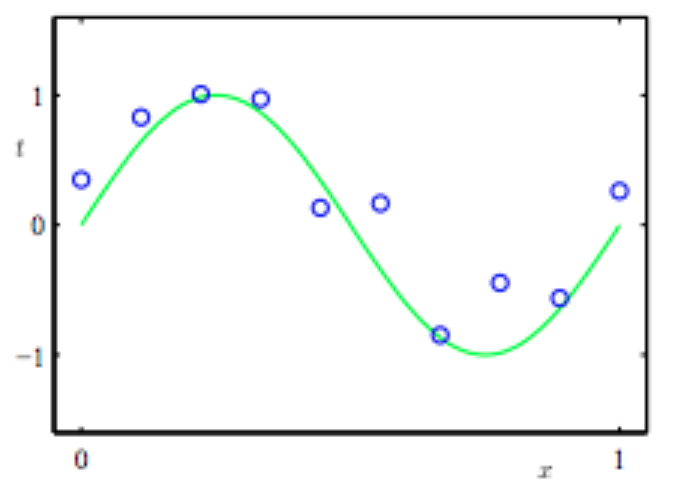
\includegraphics[width=\linewidth]{curvefitting.png}
  \caption{An example data set where we want to fit a polynomial curve into.}
\end{marginfigure}

\subsection{The Problem}\label{sec:headings}

\newthought{Suppose} we are given a training set of $N$ observations, $(x_{1},
x_{2}, \ldots, x_{N})$ and $(t_{1}, t_{2}, \ldots, x_{N})$, $x_{i}, t_{i} \in
\mathbb{R}$. We want to find a polynomial $y(x)$ that fits these data the best.

Let's start out by defining a $y(x, \mathbf{w})$.

\begin{equation}
  y(x, \mathbf{w}) = w_0 + w_1x + w_2x^2 + \ldots + w_Mx^M =
  \sum\limits_{i = 1}^M(w_ix^i)
\end{equation}

How do we measure success? Or, a better question, for what values of the
coefficients $\mathbf{w}$ will yield the best results? To answer that, we define
an error function $E$.

\begin{equation}
  E(\mathbf{w}) = \frac{1}{2}\sum\limits_{i = 1}^N(y(x_i, \mathbf{w}) - t_i)^2
\end{equation}

We then use the $\arg\min\limits_{x}f(x)$ function to find the value for the
parameter that yields the lowest value in a given function.

\begin{equation}
  \mathbf{w}^* = \arg \min\limits_{\mathbf{w}}E(\mathbf{w})
\end{equation}

$\min\limits_{x} f(x)$ finds the lowest possible value for the
expression $f(x)$, while $\arg\min\limits_{x} f(x)$ finds the value for $x$
where $f(x)$ would be the lowest.

So, in other words, we want to find a $\mathbf{w}$ such that $E(\mathbf{w})$ is
the lowest among the set of all possible values of $\mathbf{w}$.

\newthought{Except}, the attempt at finding a value $\mathbf{w}^*$ such that
$E(\mathbf{w}^*) = 0$ can become problematic.

Earlier, we mentioned that we had an initial set of training data. However, for
most cases, when trying to fit the polynomial such that $E(\mathbf{w}^*) = 0$,
for the training set, we risk having it so that when a test data set is
introduced, the error function yields a high value. This is known as
\textit{overfitting}.

\begin{marginfigure}
  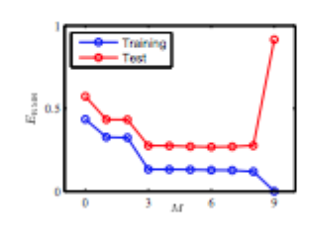
\includegraphics[width=\linewidth]{overfitting.png}
  \caption{As we can see, the first few polynomials of degree $N < 9$ fit the
    data fine, even when test data is introduced to the training set, but misses
    the mark entirely when $N = 9$. This is the result of overfitting.}
\end{marginfigure}

In the end of the day, although we want the curve to fit the data as best as
possible, we also want a \textit{genralization} derived from the given training.

\newthought{But first}, before we go ahead with finding a good gneralization,
for convenience, instead of just using the error function $E$, we use the
root-mean-square (RMS) error function, defined by

\begin{equation}
  E_{\text{RMS}} = \sqrt{2E(\mathbf{w}^*)/N}
\end{equation}

According to the text book, \textit{Pattern Recognition and Machine Learning},
the reason why we are using RMS, is the following:

\begin{quote}
  [The] division by $N$ allows us to compare different sizes of data sets
  on an equal footing, and the square root ensures that $E_{\text{RMS}}$ is
  measured on the same scale (and in the same units) as the target variable $t$.
  (p. 7)
\end{quote}

Now, to actually tune our $\mathbf{w}$ for better generalization, we can split
our training data into two sets: training set and validation set. In the case of
finding the polynomial, the training set can be used to find each $w_i \in
\mathbf{w}$, and the validation set is used to optimize the complexity, which
can be represented by $M$ (the size of $\mathbf{w}$), or a $\lambda$, which
will be discussed later.

There are several techniques used to control overfitting.

\newthought{The first technique} to avoid overfitting is cross-validation.

\begin{marginfigure}
  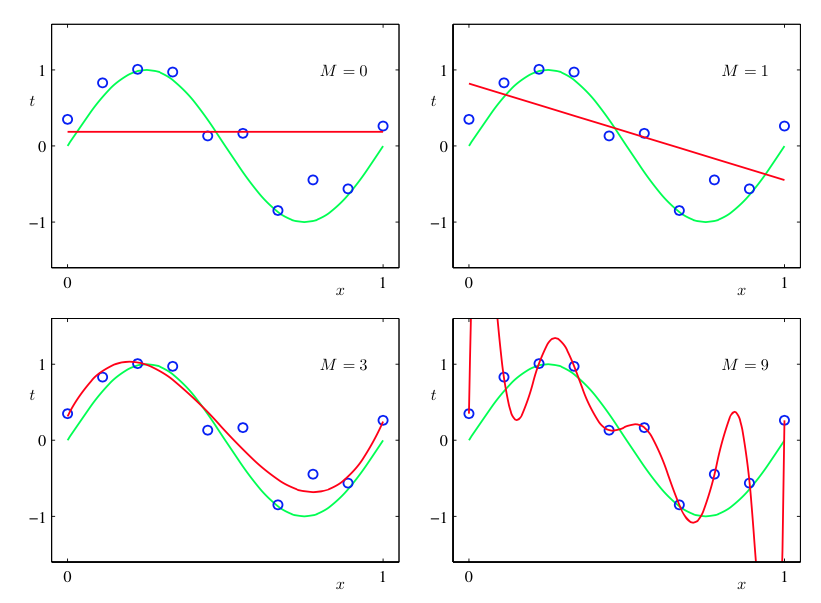
\includegraphics[width=\linewidth]{oscillations.png}
  \caption{Visually, we see that the oscillation increases as $M$ increases.}
\end{marginfigure}

Here, we group the data into separate sets. We first ``train'' our parameters to
a union of all the separated set, while leaving one out. Then we optimize by
including the one we initially excluded. Afterwards, we ``train'' again with a
new union of our sets, while leaving yet another one out, but including the one
that we initially left out, all the way until no sets are left to ``leave out''.

\newthought{And then}, there's regularization for controlling over-fitting.

Notice how the oscillation increases as $M$ increases? This is because the
magnitudes of the coefficients in $\mathbf{w}$ increases as $M$ increases.

\begin{table}[h]
  % \footnotesize%
  \begin{center}
    \begin{tabular}{lrrrr}
      \toprule
       & $M = 0$ & $M = 1$ & $M = 6$ & $M = 9$ \\
      \midrule
      $w_0$ & 0.19 &  0.82 &   0.31 &        0.35 \\
      $w_1$ &      & -1.27 &   7.99 &      232.37 \\
      $w_2$ &      &       & -25.43 &    -5321.83 \\
      $w_3$ &      &       &  17.37 &    48568.31 \\
      $w_4$ &      &       &        &  -231639.30 \\
      $w_5$ &      &       &        &   640042.26 \\
      $w_6$ &      &       &        & -1061800.52 \\
      $w_7$ &      &       &        &  1042400.18 \\
      $w_8$ &      &       &        &  -557682.99 \\
      $w_9$ &      &       &        &   125201.43 \\
      \bottomrule
    \end{tabular}
  \end{center}
  \caption{For higher values of $M$, we see the magnitude of $w_i$ increasing}
  \label{tab:font-sizes}
\end{table}

In order to avoid high coefficient magnitudes, we can ``penalize'' them using
a modified error function, by adding a $\frac{\lambda}{2}\|\mathbf{w}\|$ term
to the original error function.

\begin{equation}
  \widetilde{E}(\mathbf{w}) =
    \frac{1}{2}\sum\limits_{i = 1}^N(y(x_i, \mathbf{w}) - t_i)^2
      + \frac{\lambda}{2}\|\mathbf{w}\|
    = E(\mathbf{w}) + \frac{\lambda}{2}\|\mathbf{w}\|
\end{equation}

If we are to now apply the error function to our trials, we see that the
ceofficient are no longer large.

\begin{table}[h]
  % \footnotesize%
  \begin{center}
    \begin{tabular}{lrrr}
      \toprule
       & $\ln\lambda = -\infty$ & $\ln\lambda = -18$ & $\ln\lambda = 9$ \\
      \midrule
      $w_0$ &        0.35 &   0.35 &  0.13 \\
      $w_1$ &      232.37 &   4.74 & -0.05 \\
      $w_2$ &    -5321.83 &  -0.77 & -0.06 \\
      $w_3$ &    48568.31 & -31.93 & -0.05 \\
      $w_4$ &  -231639.30 &  -3.89 & -0.03 \\
      $w_5$ &   640042.26 &  55.28 & -0.02 \\
      $w_6$ & -1061800.52 &  41.32 & -0.01 \\
      $w_7$ &  1042400.18 & -45.95 & -0.00 \\
      $w_8$ &  -557682.99 & -91.53 &  0.00 \\
      $w_9$ &   125201.43 &  72.68 &  0.01 \\
      \bottomrule
    \end{tabular}
  \end{center}
  \caption{For higher values of $\lambda$, the coefficient magnitudes are much
    lower, possibly even near $0$}
  \label{tab:font-sizes}
\end{table}

\begin{figure*}[h] \label{}
  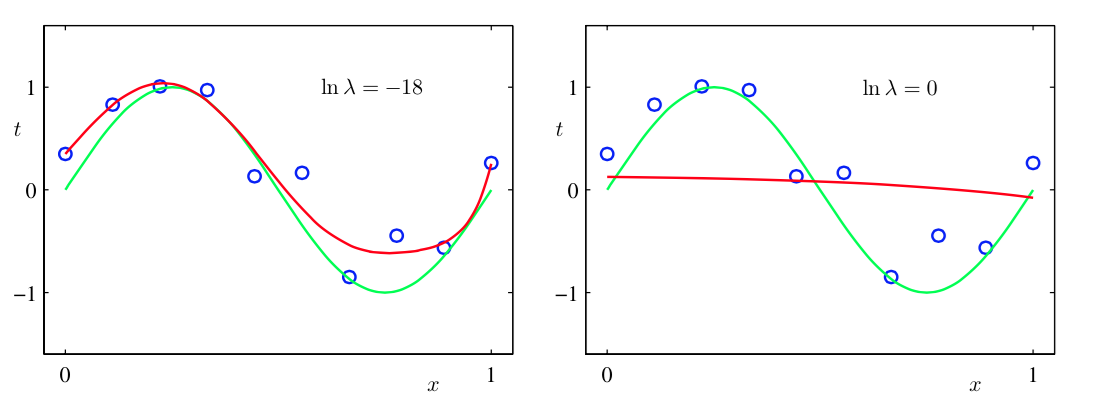
\includegraphics[width=\linewidth]{lambda.png}
  \caption{As you can see here, even for $M$ $=$ $9$,
  previously, the polynomial curve deviated wildly, which could have
  potentially yielded high error values relative to new potential data.}
\end{figure*}

\break

\newthought{Finally}, there's the third option: just get more data! A rule of
thumb is that the number of datapoints should not be any less than five times
the number of adaptive parameters.

\begin{figure*}[h]
  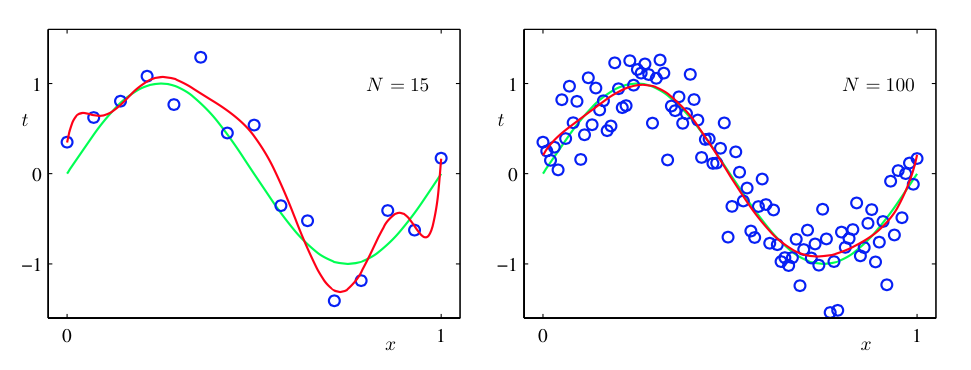
\includegraphics[width=\linewidth]{moredata.png}%
  \caption{On the left, we see an \emph{attempt} at having the curve fitted to
  the data we have so far; on the right, we see more data added, and the curve
  appears show a much better approximation.}
\end{figure*}

\break

\section{Probability Theory}

\newthought{In probability}, we have a function $p$ that returns a probability
of a given event $E$, in the range between $0$ and $1$.

\begin{equation}
  p(E) \in [0, 1]
\end{equation}
\sidenote{The prof during lecture said that $P(E) \in \mathbb{R}$.}

We can express E as just about anything.

\begin{align}
  & p(\text{Rains tomorrow}) \\
  & p(\text{Sunny tomorrow}) \\
  & p(\text{I win the lottery})
\end{align}

And also, we denote the probability of an event \emph{not} happening as the
subtraction

\begin{equation} \label{equation:probabilitynot}
  p(\text{not } E) = 1 - p(E)
\end{equation}

\subsection{Random Variables}

\newthought{If we have} a list of possible events that we want to plug in to
$p$, we use what is called a ``random variable''.

The term ``random variable'' can be misleading. A random variable is not a
variable at all. Instead, it's a mapping from a \emph{random event} to a
possible outcome.

So here's an example random variable:

\begin{equation}
  X =
    \begin{cases}
      1 \text{ if } \text{heads} \\
      0 \text{ if } \text{tails} \\
    \end{cases}
\end{equation}

As we can see here, $X$ is a mapping from the set $\{ \text{heads},
\text{tails} \}$, to the set $\{ 1, 0 \}$. Bear in mind, although the above
example is showing a mapping of only two elements, a random variable can consist
of many more.

More informally, a random variable is a ``label'' to a given element of a set of
possible events.

To add to the confusion, when we say that we have an event from our random
variable (for example, an event from $X$ defined above), we express it as
$X = 0$ or $X = 1$, etc.

The end purpose of random variables is to derive a probability distribution
given a value $x \in \{ \text{Range of X} \}$. So, going back to the above
head/tail example, if we wanted to express the probability of getting heads, we
write $p(X = 1)$, likewise, for expressing the probability of getting tails, we
write $p(X = 0)$, and so and so forth.

The other purpose of using random variables is for us to easily be able to
express multiple events concisely.

For example, let's define a random variable $Y$ that contains a mapping of a
list of events given by the sum of the faces of two dice rolls. Let's say we
wanted to find the probability of the event that the faces of the two dice rolls
sum to $10$ or less. Instead of writing every single possible event---
e.g. $p(Y = 2 \text{ or } Y = 3 \text{ or } \ldots \text{ or } Y = 10)$---we can
simply express the event as an inequality, e.g. $p(Y \leq 10)$.

\subsection{More on Probability}

\newthought{Imagine} a grid formed from the values in the random variable $X$
and values in the random variable $Y$, where $x_i \in \{\text{Range of } X\}$,
and where $y_j \in \{\text{Range of } Y\}$, and $i \in \{ 1, 2, \ldots, M \}$,
and $j \in \{ 1, 2, \ldots, L \}$. $X$ represents the rows, and $Y$ represents
the columns \sidenote{In the textbook, $X$ represents the columns and $Y$
represents the rows. Why did I set $X$ to be the rows, $Y$ as the columns? It
was a total mistake on my part. I'm not gonna change it, though; too much time
needed. Either ways, trying to mentally remap between the textbook and these
notes is good excercise anyways}. The total number of trials is $N = ML$. We
will express a single trial as $n_{ij}$.

For the probability that we get a row $x_i$, we express $p(X = x_i)$, and for
column $y_j$, we express $p(Y = y_j)$. Evaluating the probability for $X$ and
$Y$, we get:

\begin{equation} \label{equation:probbasic}
  p(X = x_i) = \frac{r_i}{N}, p(Y = y_j) = \frac{c_j}{N}
\end{equation}

\sidenote{N.B. the value $r_i$ and $c_j$ are not same as
evaluating $n_{ij}$.}

Now, let's say we are to evaluate the probability that we get a specific column,
and a specific row, we write $p(X = x_i, Y = y_i)$. This is known as a
\emph{joint probability}. Evaluating for $X$ \emph{and} $Y$, we get:

\begin{equation} \label{equation:jointprob}
  p(X = x_i, Y = y_j) = \frac{n_{ij}}{N}
\end{equation}

Notice how we get back $n_{ij}$? This is true even if we are to flip the
parameters in $p(\cdot, \cdot)$. And so, joint probabilities are symmetric,

\begin{equation}\label{equation:probabilitysymmetry}
  p(X = x_i, Y = y_j) = p(Y = y_j, X = x_i)
\end{equation}

So now, let's go back to columns and rows. To expand on $p(X = x_i)$, we can
alternatively evaluate it as:

\begin{equation}
  p(X = x_i) = \sum\limits_{j = 1}^Lp(X = x_i, Y = y_j)
\end{equation}

Likewise, for $p(Y = y_j)$:

\begin{equation}
  p(Y = y_j) = \sum\limits_{i = 1}^Mp(X = x_i, Y = y_j)
\end{equation}

\sidenote{$p(X = x_i)$ and $p(Y = y_j)$ are known as marginal probabilities.}

The above equation expresses the ``sum rule''.

Let's simplify our probability expression. Often times, when we look at the
event $X = x_i$, we are saying that there exists an $x_i$ from $X$, but in the
end of the day, we simply don't care about the value of $x_i$. In this case we
can simplify the expression to write $p(X)$.

\newthought{Now, let's talk about} conditional probability. With conditional
probability, we can concisely express the probability of some event \emph{given}
some other event. With events $X$ and $Y$, we express the probability that we
get $X$ given $Y$ as $p(X|Y)$. Because we are narrowing our list of
probabilities down to a specific column ($Y$), then instead of having our
probability be the ratio over $N$, we have it be the the ratio over the
probability of getting some column.

\begin{equation} \label{equation:conditionalprob}
  p(X = x_i | Y = y_j) = \frac{n_{ij}}{c_i}
\end{equation}

From (\ref{equation:probbasic}), (\ref{equation:jointprob}), and
(\ref{equation:conditionalprob}), we can derive the following relationship:

\begin{equation}
  \begin{aligned}
    p(X = x_i , Y = y_j) &= \frac{n_{ij}}{N} = \frac{n_{ij}}{c_i} \cdot \frac{c_i}{N} \\
                         & = p(X = x_i | Y = y_j)p(Y = y_i)
  \end{aligned}
\end{equation}

Which is known as the \emph{product rule} of probability.

\begin{tcolorbox}
  The Rules of Probability
  \begin{align}
    p(X) &= \sum\limits_{Y}p(X, Y) & \text{    Sum Rule} \label{equation:sumrule}\\
    p(X, Y) &= p(Y|X)p(X) & \text{    Product Rule} \label{equation:productrule}
  \end{align}
\end{tcolorbox}

According to (\ref{equation:productrule}), we can rewrite the $p(X, Y)$ in
(\ref{equation:sumrule}) to:

\begin{equation}
  p(X) = \sum\limits_{Y}p(X, Y) = \sum\limits_{Y}p(Y|X)p(X)
\end{equation}

And also, because of (\ref{equation:probabilitysymmetry}), according to
(\ref{equation:productrule}), we can rewrite $p(X, Y) = p(Y, X)$ to:

\begin{equation}\label{equation:alternatesymmetry}
  p(Y|X)p(X) = p(X|Y)p(Y)
\end{equation}

And, we can then isolate $p(Y|X)$ in (\ref{equation:alternatesymmetry})

\begin{equation}
  p(Y|X) = \frac{p(X|Y)p(Y)}{p(X)}
\end{equation}

Which is known as \emph{Bayes' Theorem}.

\subsection{Bayesian Thinking}

\newthought{To get the motivation} behind Bayes' Theorem, let's think about a
real world scenario where we can apply Bayesian Thinking.

Let's say we had two boxes, coloured red and blue. The probability of getting
red is 40\%, and the probability of getting blue is 60\%. The box events will
be represented by the random variable $B$. We will be abbreviating ``red'' with
$r$ and ``blue'' with $b$. We would respectively denote them as

\begin{align}
  p(B = r) &= 0.4 \\
  p(B = b) &= 0.6
\end{align}

Both the boxes have a specific number of apples and oranges. The red one has
two apples and six oranges, and the blue one has three apples and one orange.
The fruit events will be represented by the random variable $F$. We will also
be abbreviating ``apple'' with $a$ and ``orange'' with $o$.

\begin{marginfigure}
  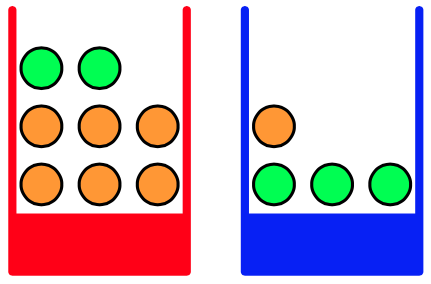
\includegraphics[width=\linewidth]{fruitboxes.png}
  \caption{The distribution of fruits in our boxes.}
\end{marginfigure}

The probability distribution of each boxes would look like so:

\begin{align}
  p(F = a | B = r) &= 0.25 \\
  p(F = o | B = r) &= 0.75 \\
  p(F = a | B = b) &= 0.75 \\
  p(F = o | B = b) &= 0.25
\end{align}

Then, to find the probability of choosing an apple overall, we simply apply the
sum and product rule.

\begin{equation}
  \begin{aligned}
    p(F = a) &= p(F = a|B = r)p(B = r) + p(F = a|B = b)p(B = b)\\
             &= 0.25 \times 0.4 + 0.75 \times 0.6 \\
             &= 0.55
  \end{aligned}
\end{equation}

Since there are only apples and oranges, we can argue that the probability that
we pick an orange is equally the probability of \emph{not} picking an apple. And
so by (\ref{equation:probabilitynot}), we can concisely find the probability of
picking an orange with $p(F = o) = p(F \neq a) = 1 - p(F = a)$ = 0.45.

Let's say we were asked from which box we had picked a fruit. Without knowing
what fruit we picked, we only know the probability of the box, which is $p(B)$.
This is called the \emph{prior probability}. Now, we find out that the fruit
that we picked was an orange, and we now have a probability $p(B|F)$, which is
called the \emph{posterior probability}. In Bayes' theorem, we take the prior
and multiply it with the probability of picking orange given the box, $p(F|B)$.
$p(F|B)$ is called the \emph{likelihood}. Because we want to find the
probability of a box given a fruit, we narrow the product $p(F|B)p(B)$ by dividing by
$p(F)$.

So to summarize:

\begin{equation}
  p(B|F) = \frac{p(F|B)p(B)}{p(F)}
\end{equation}

Given the above equation, we find that we are more likely to pick from the red
box, given the fruit is an orange. I will leave it to you to verify.

\subsection{Some stuff about Bernoulli trials}

% \sidenote{I have no clue why the following
% was in my notebook. Regardless, I have typed out the following, in order to
% avoid the risk of losing any of it, in case my notebook burns up somehow.}:

\newthought{Earlier}, we talked about probabilities in general, as well as
bayes theorem. Here, we are going to talk about probabilities of random
variables that only have two events, and two events only. We are going to talk
about Bernoulli trials.

Let's say we had two events, $a$ and $b$, such that it has the following
probability distributions

\begin{equation}
  \begin{aligned}
    p(a) &= \mu \\
    p(b) &= 1 - \mu
  \end{aligned}
\end{equation}

Now, let's define a $\mathcal{D} = \{x_1, x_2, \ldots, x_N\}$, such that it
contains an arbitrary $N$ number of events of either $a$ or $b$, except, let's
replace the event $a$ to equal $1$, and $b$ to equal $0$.

To get the probability of $\mathcal{D}$, we have the probabilities of $a$ and
$b$, and so, for each element of $\mathcal{D}$, we have some $\mu$ that dictates
whether the said element is $a$, or $b$.

A concise way to express the above would be $p(\mathcal{D}|\mu)$.

It gets even better. Notice how we defined $a = 1$, and $b = 0$? And also,
$p(a) = \mu$ and $p(b) = 1 - \mu$. Let's define a $c$ so that it is either $a$
or $b$. This means we can generalize $p(a)$ and $p(b)$ so that
$p(c) = \mu^c(1 - \mu)^c$. And remember, since $c$ can either $a$ or $b$; this
ultimately means that $c$ can either by $0$ or $1$!

And so, expanding $p(\mathcal{D}|\mu)$, we get

\begin{equation} \label{equation:bernoulliequation}
  \begin{aligned}
    p(\mathcal{D}|\mu) &= p(\{x_1, x_2, \dots, x_N\}|\mu) \\
                       &= p(x_1|\mu) \cdot p(x_2|\mu) \cdot \ldots \cdot p(x_N|\mu) \\
                       &= \prod_{i = 1}^N p(x_i|\mu) \\
                       &= \prod_{i = 1}^N \mu x^i(1 - \mu)^{1 - x_i}
  \end{aligned}
\end{equation}

Now, we need to find a $\mu$ that will be the highest possible value for the
expressesion $p(\mathcal{D}|\mu)$. In other words, we want to compute

\begin{equation}
  \mu* = \arg \max\limits_{\mu}p(\mathcal{D}|\mu)
\end{equation}

How will we achieve?

First, let's go back to (\ref{equation:bernoulliequation}), and solve for $\mu$.

However, it's going to be very difficult to solve given the fact that 1), each
of the probabilities are multiplacands, 2) the $\mu$s have an exponent attached.

Fortunately, there's a postulate

\begin{equation} \label{equation:lnidentity}
  \begin{aligned}
    \arg \max\limits_x f(x) = \arg\max\limits_x \ln f(x) \\
    f(x) \in \{\text{monotonically increasing}\}
  \end{aligned}
\end{equation}

And so, this means that we can compute $\ln p(\mathcal{D}|\mu)$, and then 1)
convert the products into sums, and 2) eliminate the exponent by getting the
derivative, making it easier to solve for $\mu$.

\begin{equation}
  \begin{aligned}
    0 = p(\mathcal{D}|\mu)              &= \prod\limits_{i = 1}^N \mu^{x_i}(1 - \mu)^{1 - x_i} \rightarrow \\
    \ln p(\mathcal{D}|\mu)              &= \ln \prod\limits_{i = 1}^N \mu^{x_i}(1 - \mu)^{1 - x_i} \\
                                        &= \sum\limits_{i = 1}^N \ln \mu^{x_i}(1 - \mu)^{1 - x_i} \\
                                        &= \sum\limits_{i = 1}^N x^i \ln \mu + (1 - x_i)\ln (1 - \mu) \rightarrow \\
    \frac{d}{dx} \ln p(\mathcal{D}|\mu) &= \frac{d}{dx} \sum\limits_{i = 1}^N x^i \ln \mu + (1 - x_i)\ln (1 - \mu) \\
                                        &= \sum\limits_{i = 1}^N \frac{x_i}{\mu} - \frac{1 - x_i}{1 - \mu} \\
                                        &= \frac{1}{\mu} (\sum\limits_{i = 1}^N x_i) - \frac{1}{1 - \mu}(\sum\limits_{i = 1}^N1 - x_i)
  \end{aligned}
\end{equation}

And then, we substitute $\sum\limits_{i = 1}^Nx_i$ for an unknown $h$, and
replace $\sum\limits_{i = 1}^N1-x_i$ for an unknown t, and finally isolate $\mu$.

\begin{equation}
  \begin{aligned}
    \frac{d}{dx} \ln p(\mathcal{D}|\mu) = 0 &= \frac{h}{\mu} - \frac{t}{1 - \mu} \rightarrow \\
    % 0 &= \frac{h}{\mu} - \frac{t}{1 - \mu} \rightarrow \\
    \mu &= \frac{h}{h + t}
  \end{aligned}
\end{equation}

% \bibliography{sample-handout}
% \bibliographystyle{plainnat}

\end{document}
